\documentclass{article}
\usepackage{amsmath,amssymb,amsthm,kotex,paralist,mathrsfs,centernot,marvosym}
\newcounter{num}
\newcommand{\defi}[1]
{\bigskip\noindent\refstepcounter{num}\textbf{정의 \arabic{num}) #1}\par}
\newcommand{\theo}[1]
{\bigskip\noindent\refstepcounter{num}\textbf{정리 \arabic{num}) #1}\par}
\newcommand{\exam}[1]
{\bigskip\noindent\refstepcounter{num}\textbf{예시 \arabic{num}) #1}\par}

\newcommand{\notiff}{%
  \mathrel{{\ooalign{\hidewidth$\not\phantom{"}$\hidewidth\cr$\iff$}}}}
\newcommand{\LHS}{\text{LHS}}
\newcommand{\RHS}{\text{RHS}}
\newcommand{\irange}{\ensuremath{1\le i\le n}}
\newcommand{\jrange}{\ensuremath{1\le j\le n}}


%%%
\begin{document}

\title{현빈 : 12 등차수열과 등비수열}
\author{}
\date{\today}
\maketitle

%
\defi{수열}
\(3\), \(6\), \(9\), \(12\), \(\cdots\)와 같이 어떤 일정한 규칙에 따라 차례로 나열된 수의 열을 수열(sequence)이라고 하고 나열된 각각의 수를 항(term)이라 한다.

\defi{수열의 일반항}
수열을 \(a_1\), \(a_2\), \(a_3\), \(\cdots\), \(a_n\), \(\cdots\)으로 나타낼 때 각각의 수를 항이라 하고 처음부터 차례로 \(a_1\)을 첫째항, \(a_2\)를 둘째항, \(\cdots\), \(a_n\)을 \(n\)째항 이라고 한다. 특히 \(n\)째항인 \(a_n\)을 일반항이라고 한다.
수열을 나타낼 때에는 \(\{a_n\}\)과 같이 나타낸다.

예를 들어, 앞서 언급한 \(3\), \(6\), \(9\), \(12\), \(\cdots\)에서 \(a_1=3\), \(a_2=6\), \(a_3=9\), \(a_4=12\), \(\cdots\), \(a_n\), \(\cdots\)이므로 수열의 일반항은 \(a_n=3n\)이다.

\section{등차수열}

\defi{등차수열}
수열 \(3\), \(6\), \(9\), \(12\), \(\cdots\)와 같이, 첫째항부터 차례로 일정한 수를 더해서 얻어지는 수열을 등차수열(Arithmetic Progression)이라고 하고 그 일정한 수를 공차라고 한다.

\exam{등차수열의 예}
다음 수열들은 모두 등차수열이다.
\begin{align}
3, 6, 9, 12, \cdots\:;\quad	&\text{첫째항=}3\:;\quad		\text{공차=}3\:;\quad a_n=3n\\
1, 3, 5, 7, \cdots\:;\quad		&\text{첫째항=}1\:;\quad		\text{공차=}2\:;\quad a_n=2n-1\\
1, 1, 1, 1, \cdots\:;\quad		&\text{첫째항=}1\:;\quad		\text{공차=}0\:;\quad a_n=1\\
-1, -2, -3, -4, \cdots\:;\quad	&\text{첫째항=}-1\:;\quad	\text{공차=}-1\:;\quad a_n=-n\\
-4, -2, 0, 2, \cdots\:;\quad	&\text{첫째항=}-4\:;\quad	\text{공차=}2\:;\quad a_n=2n-6\\
\frac23, \frac13, 0, -\frac13, \cdots\:;\quad
				&\text{첫째항=}\frac23\:;\quad\text{공차=}-\frac13\:;\quad a_n=-\frac13+1
\end{align}

%\theo{등차수열의 일반항}
%등차수열 \(\{a_n\}\)의 첫항을 \(a\), 공차를 \(d\)라고 하면 \(a_1=a\), \(a_2=a+d\), \(a_3=a+2d\), \(a_4=a+3d\), \(\cdots\)이다.
%일반적으로
%\[a_n=a+(n-1)d\]
%이다.

\exam{등차수열의 합}
\(a_n=3n+1\)로 주어진 등차수열 \(\{a_n\}\)에 대해 10항까지의 합을 \(S\)라고 하자(S=\(a_1+a_2+a_3+\cdots+a_{10}\)).
그러면 \(S\)는 다음과 같이 구할 수 있다.

일단 \(S\)를 정의에 맞게 쓰면
\[
S=4+7+10+\cdots+25+28+31
\]
이다.
이 식에서 나열된 수의 순서를 바꾸면
\[
S=31+28+25+\cdots+10+7+4
\]
이다.
이 두 식을 더하면
\begin{align*}
2S
&=(4+31)+(7+28)+(10+25)+\cdots+(25+10)+(28+7)+(31+4)\\
&=35+35+\cdots+35\\
&=35\times10=350
\end{align*}
이다.
따라서
\[S=175.\]

\bigskip\bigskip
--------------------- 예 제 ---------------------

02.
다음 등차수열의 일반항 \(a_n\)을 구하여라.

\quad\:
(1) \(-11\), \(-8\), \(-5\), \(-2\), \(\cdots\)

\quad\:
(2) \(6\), \(3\), \(0\), \(-3\), \(\cdots\)

\bigskip
09.
다음 등차수열의 합을 구하여라.

\quad\:
(1) \(a_n=2n+1\), 10째항까지

\quad\:
(3) \(a_n=2n+5\), 33항까지

\bigskip\bigskip
--------------------- 연습 문제 ---------------------

194.
다음은 등차수열이다. \(\square\)안에 알맞은 수를 써넣어라.

\quad\:
(1) \(6\), \(0\), \(-6\), \(\square\), \(\square\)

\quad\:
(2) \(\square\), \(15\), \(\square\), \(27\)

\quad\:
(3) \(\frac34\), \(\frac14\), \(-\frac14\), \(\square\), \(\square\)

\quad\:
(4) \(\square\), \(\frac13\), \(\frac12\), \(\square\)

\bigskip
195.
다음 등차수열의 일반항 \(a_n\)을 구하여라.

\quad\:
(1) \(3\), \(6\), \(9\), \(\cdots\)

\quad\:
(2) \(10\), \(7\), \(4\), \(1\), \(\cdots\)

\bigskip
196.
일반항 \(a_n\)이 다음과 같은 등차수열의 첫째항과 공차를 구하여라.

\quad\:
(1) \(a_n=3n+5\)

\quad\:
(2) \(a_n=-7n+9\)

\bigskip
196*.
일반항 \(a_n\)이 다음과 같은 등차수열의 10항까지의 합을 구하여라.

\quad\:
(1) \(a_n=3n+5\)

\quad\:
(2) \(a_n=-7n+9\)

\bigskip\bigskip
--------------------- 추가문제 ---------------------

217.
어느 프로야구 투수는 시즌 개막 한 달 전부터 개막전에 대비해 매일 투구 수를 늘려가며 연습을 해왔다고 한다. 첫째 날 50개, 둘째 날 52개, 셋재 날 54개, \(\cdots\)와 같이 매일 2개씩 늘려가며 30일간 연습을 했다면 연습한 투구 수는 총 몇 개인가?

\bigskip
220.
등차수열 \(\{a_n\}\)에서 \(a_5+a_{15}=10\)일 때, \(a_3+a_7+a_{10}+a_{13}+a_{17}\)의 값을 구하여라.

\bigskip
232.
다음 그림에서 가로줄과 세로줄에 있는 세 수가 각각 등차수열을 이룬다.
예를 들어 \(a\), \(b\), \(2\)는 이 순서대로 등차수열을 이루고, \(b\), \(c\), \(6\)은 이 순서대로 등차수열을 이룬다.
이때 \(a+b-(d+f)\)의 값을 구하여라.

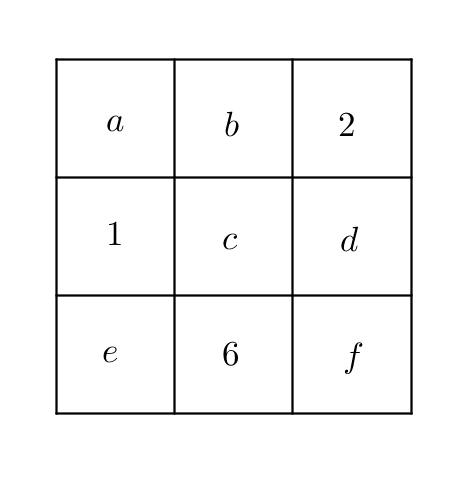
\includegraphics{232}

%
\section{등비수열}

\defi{등비수열}
수열 \(1\), \(2\), \(4\), \(8\), \(\cdots\)와 같이, 첫째항부터 차례로 일정한 수를 곱해서 얻어지는 수열을 등비수열(Geometric Progression)이라고 하고 그 일정한 수를 공비라고 한다.

\exam{등비수열의 예}
다음 수열들은 모두 등차수열이다.
\begin{align}
1, 2, 4, 8, \cdots\:;\quad		&\text{첫째항=}1\:;	\quad	\text{공비=}2\:;\quad a_n=2^{n-1}\\
3, 9, 27, 81, \cdots\:;\quad	&\text{첫째항=}3\:;	\quad	\text{공비=}3\:;\quad a_n=3^n\\
3, 6, 12, 24, \cdots\:;\quad&\text{첫째항=}3\:;\quad\text{공비=}2\:;\quad a_n=3\cdot2^{n-1}\\
2,-4,8,-16, \cdots\:;\quad&\text{첫째항=}2\:;\quad	\text{공비=}-2\:;\quad a_n=2\cdot(-2)^{n-1}\\
-1, 1, -1, 1, \cdots\:;\quad	&\text{첫째항=}-1	\:;\quad	\text{공비=}-1\:;\quad a_n=(-1)^n\\
\frac23, 1, \frac32, \frac94, \cdots\:;\quad	&\text{첫째항=}\frac23\:;
\quad\text{공차=}\frac32\:;\quad a_n=\frac49\left(\frac32\right)^{n-1}
\end{align}

%\theo{등차수열의 일반항}
%등차수열 \(\{a_n\}\)의 첫항을 \(a\), 공차를 \(d\)라고 하면 \(a_1=a\), \(a_2=a+d\), \(a_3=a+2d\), \(a_4=a+3d\), \(\cdots\)이다.
%일반적으로
%\[a_n=a+(n-1)d\]
%이다.

\exam{등비수열의 합}
\(a_n=3^n\)로 주어진 등비수열 \(\{a_n\}\)에 대해 10항까지의 합을 \(S\)라고 하자(S=\(a_1+a_2+a_3+\cdots+a_{10}\)).
그러면 \(S\)는 다음과 같이 구할 수 있다.

일단 \(S\)를 정의에 맞게 쓰면
\[
S=3+3^2+3^3+\cdots+3^8+3^9+3^{10}
\]
이다.
이 식의 양변에 공비(=3)을 곱하면
\[
3S=3^2+3^3+3^4+\cdots+3^9+3^{10}+3^{11}
\]
이다.
이 두 식의 차이를 계산하면
\begin{align*}
2S
&=(3^2+3^3+3^4+\cdots+3^9+3^{10}+3^{11})-(3+3^2+3^3+\cdots+3^8+3^9+3^{10})\\
&=3^{11}-3
\end{align*}
따라서
\[S=\frac12(3^{11}-3)\]

\bigskip\bigskip
--------------------- 예 제 ---------------------

16.
다음 등비수열의 일반항 \(a_n\)을 구하여라.

\quad\:
(1) \(-2\), \(4\), \(-8\), \(16\), \(\cdots\)

\quad\:
(2) \(9\), \(-3\), \(1\), \(-\frac13\), \(\cdots\)

\quad\:
(3) \(1\), \(-\frac1{\sqrt3}\), \(\frac13\), \(\cdots\)

\bigskip
17.
다음 물음에 답하여라.

\quad\:
(1) 등비수열 \(4\), \(-12\), \(36\), \(-108\), \(\cdots\)에서 \(-972\)는 몇 번째 항인지 구하여라.

\quad\:
(2) 공비가 \(-2\), \(a_6=-160\)인 등비수열의 첫째항을 구하여라.

\bigskip
18.
\(a_n=3\cdot2^{1-2n}\)인 등비수열 \(\{a_n\}\)의 첫째항과 공비를 구하여라.

24.
다음 수열의 합을 구하여라.

\quad\:
(1) \(3\), \(6\), \(12\), \(24\), \(\cdots\) (제 10 항까지)

\quad\:
(2) \(1\), \(\frac13\), \(\frac19\), \(\cdots\) (제 \(n\) 항까지)

\quad\:
(3) \(1-2+4-\cdots-512\)

\bigskip\bigskip
--------------------- 연습문제 ---------------------

215.
다음 등비수열 \(\{a_n\}\)의 \(\square\) 안에 알맞은 수를 써넣어라.

\quad\:
(1) \(\square\), \(\square\), \(18\), \(-54\), \(\cdots\)

\quad\:
(2) \(\sqrt2\), \(-1\), \(\frac1{\sqrt2}\), \(\square\), \(\square\), \(\cdots\)

\bigskip
217.
등비수열 \(1\), \(-4\), \(16\), \(-64\), \(\cdots\)에서 \(-1024\)는 몇 번째 항인지 구하여라.

\bigskip
218.
\(a_n=2^{2-n}\)인 등비수열 \(\{a_n\}\)에서 첫째항과 공비를 구하여라.

\bigskip
226.
다음 수열의 합을 구하여라.

\quad\:
(1) \(1\), \(-3\), \(9\), \(-27\), \(\cdots\) (제 \(n\) 항까지)

\quad\:
(2) \(\sqrt2\), \(2\), \(2\sqrt2\), \(4\), \(\cdots\), (제 10 항까지)

\quad\:
(3) \(3+6+12+\cdots+96\)

\bigskip\bigskip
--------------------- 추가문제 ---------------------

246.
다음을 계산하여라.

\[0.3+0.03+0.003+\cdots+3\cdot\left(\frac1{10}\right)^n\]

\bigskip
247.
다음 등비수열의 합을 구하여라.
\[2^7+2^6+2^5+2^4+\cdots+2^{-8}\]

\section{멱급수}
\defi{멱급수}
수열의 합을 `급수'라고 한다.
그 중에서
\[1\cdot3+2\cdot3^2+3\cdot3^3+4\cdot3^4+\cdots n+\cdot3^n+\cdots\]
와 같이 등차수열(\(1\), \(2\), \(3\), \(\cdots\))과 등비수열(\(3\), \(3^2\), \(3^3\), \(\cdots\))이 곱해진 수열의 합을 일컫어 멱급수라고 한다.

\exam{멱급수 구하기}
위에 정의된 멱급수에서 10항까지의 합을 구해보자.
\[S=1\cdot3+2\cdot3^2+3\cdot3^3+4\cdot3^4+\cdots+10\cdot3^{10}\]
이라고 하자.
등비급수의 합을 구할 때와 마찬가지로, 등비급수의 공비인 3을 양변에 곱하면
\[3S=1\cdot3^2+2\cdot3^3+3\cdot3^4+4\cdot3^5+\cdots+10\cdot3^{11}\]
이다.

양변의 차를 구하면
\[-2S=3+3^2+3^3+\cdots+3^{10}-10\cdot3^{11}\]
이다.

\[3+3^2+3^3+\cdots+3^{10}=\frac12(3^{11}-3)\]
이므로
\[-2S=\frac12(3^{11}-3)-10\cdot3^{11}\]
이다.
이것을 정리하면
\[S=-\frac12\left[\frac12(3^{11}-3)-10\cdot3^{11}\right]\]


\end{document}